% Created by tikzDevice version 0.12
% !TEX encoding = UTF-8 Unicode
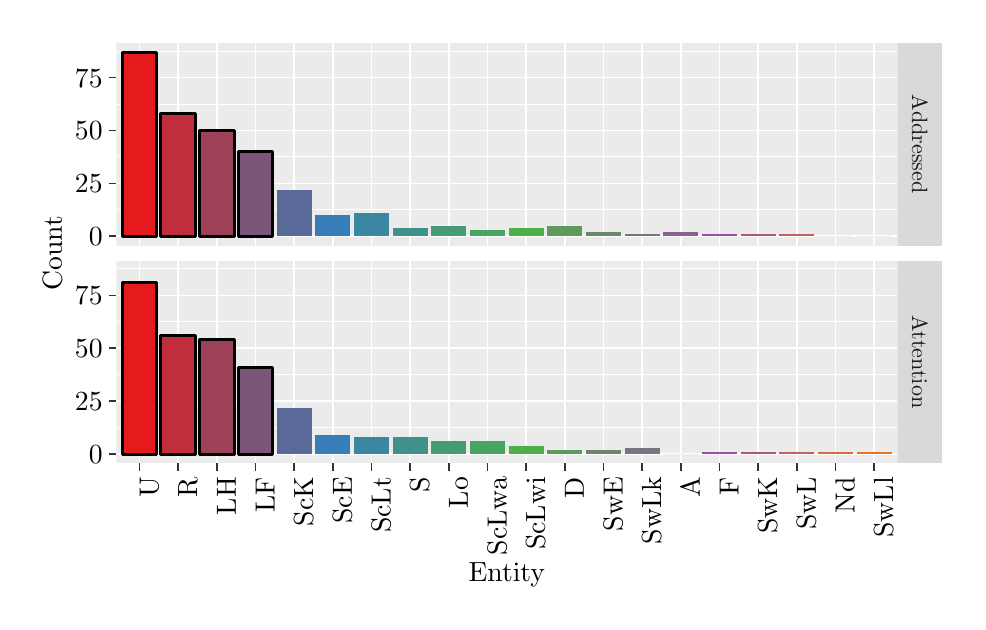
\begin{tikzpicture}[x=1pt,y=1pt]
\definecolor{fillColor}{RGB}{255,255,255}
\path[use as bounding box,fill=fillColor,fill opacity=0.00] (0,0) rectangle (336.00,207.65);
\begin{scope}
\path[clip] (  0.00,  0.00) rectangle (336.00,207.65);
\definecolor{drawColor}{RGB}{255,255,255}
\definecolor{fillColor}{RGB}{255,255,255}

\path[draw=drawColor,line width= 0.6pt,line join=round,line cap=round,fill=fillColor] (  0.00,  0.00) rectangle (336.00,207.65);
\end{scope}
\begin{scope}
\path[clip] ( 32.03,128.93) rectangle (314.25,202.15);
\definecolor{fillColor}{gray}{0.92}

\path[fill=fillColor] ( 32.03,128.93) rectangle (314.25,202.15);
\definecolor{drawColor}{RGB}{255,255,255}

\path[draw=drawColor,line width= 0.3pt,line join=round] ( 32.03,141.82) --
	(314.25,141.82);

\path[draw=drawColor,line width= 0.3pt,line join=round] ( 32.03,160.95) --
	(314.25,160.95);

\path[draw=drawColor,line width= 0.3pt,line join=round] ( 32.03,180.08) --
	(314.25,180.08);

\path[draw=drawColor,line width= 0.3pt,line join=round] ( 32.03,199.20) --
	(314.25,199.20);

\path[draw=drawColor,line width= 0.6pt,line join=round] ( 32.03,132.26) --
	(314.25,132.26);

\path[draw=drawColor,line width= 0.6pt,line join=round] ( 32.03,151.39) --
	(314.25,151.39);

\path[draw=drawColor,line width= 0.6pt,line join=round] ( 32.03,170.51) --
	(314.25,170.51);

\path[draw=drawColor,line width= 0.6pt,line join=round] ( 32.03,189.64) --
	(314.25,189.64);

\path[draw=drawColor,line width= 0.6pt,line join=round] ( 40.41,128.93) --
	( 40.41,202.15);

\path[draw=drawColor,line width= 0.6pt,line join=round] ( 54.38,128.93) --
	( 54.38,202.15);

\path[draw=drawColor,line width= 0.6pt,line join=round] ( 68.35,128.93) --
	( 68.35,202.15);

\path[draw=drawColor,line width= 0.6pt,line join=round] ( 82.32,128.93) --
	( 82.32,202.15);

\path[draw=drawColor,line width= 0.6pt,line join=round] ( 96.30,128.93) --
	( 96.30,202.15);

\path[draw=drawColor,line width= 0.6pt,line join=round] (110.27,128.93) --
	(110.27,202.15);

\path[draw=drawColor,line width= 0.6pt,line join=round] (124.24,128.93) --
	(124.24,202.15);

\path[draw=drawColor,line width= 0.6pt,line join=round] (138.21,128.93) --
	(138.21,202.15);

\path[draw=drawColor,line width= 0.6pt,line join=round] (152.18,128.93) --
	(152.18,202.15);

\path[draw=drawColor,line width= 0.6pt,line join=round] (166.15,128.93) --
	(166.15,202.15);

\path[draw=drawColor,line width= 0.6pt,line join=round] (180.12,128.93) --
	(180.12,202.15);

\path[draw=drawColor,line width= 0.6pt,line join=round] (194.09,128.93) --
	(194.09,202.15);

\path[draw=drawColor,line width= 0.6pt,line join=round] (208.07,128.93) --
	(208.07,202.15);

\path[draw=drawColor,line width= 0.6pt,line join=round] (222.04,128.93) --
	(222.04,202.15);

\path[draw=drawColor,line width= 0.6pt,line join=round] (236.01,128.93) --
	(236.01,202.15);

\path[draw=drawColor,line width= 0.6pt,line join=round] (249.98,128.93) --
	(249.98,202.15);

\path[draw=drawColor,line width= 0.6pt,line join=round] (263.95,128.93) --
	(263.95,202.15);

\path[draw=drawColor,line width= 0.6pt,line join=round] (277.92,128.93) --
	(277.92,202.15);

\path[draw=drawColor,line width= 0.6pt,line join=round] (291.89,128.93) --
	(291.89,202.15);

\path[draw=drawColor,line width= 0.6pt,line join=round] (305.86,128.93) --
	(305.86,202.15);
\definecolor{drawColor}{RGB}{0,0,0}
\definecolor{fillColor}{RGB}{228,26,28}

\path[draw=drawColor,line width= 1.1pt,line join=round,fill=fillColor] ( 34.12,132.26) rectangle ( 46.70,198.82);
\definecolor{fillColor}{RGB}{193,46,59}

\path[draw=drawColor,line width= 1.1pt,line join=round,fill=fillColor] ( 48.10,132.26) rectangle ( 60.67,176.63);
\definecolor{fillColor}{RGB}{158,66,90}

\path[draw=drawColor,line width= 1.1pt,line join=round,fill=fillColor] ( 62.07,132.26) rectangle ( 74.64,170.51);
\definecolor{fillColor}{RGB}{124,86,121}

\path[draw=drawColor,line width= 1.1pt,line join=round,fill=fillColor] ( 76.04,132.26) rectangle ( 88.61,162.86);
\definecolor{fillColor}{RGB}{89,106,152}

\path[fill=fillColor] ( 90.01,132.26) rectangle (102.58,149.09);
\definecolor{fillColor}{RGB}{55,126,184}

\path[fill=fillColor] (103.98,132.26) rectangle (116.55,139.91);
\definecolor{fillColor}{RGB}{59,135,162}

\path[fill=fillColor] (117.95,132.26) rectangle (130.53,140.68);
\definecolor{fillColor}{RGB}{63,145,139}

\path[fill=fillColor] (131.92,132.26) rectangle (144.50,135.32);
\definecolor{fillColor}{RGB}{68,155,117}

\path[fill=fillColor] (145.89,132.26) rectangle (158.47,136.09);
\definecolor{fillColor}{RGB}{72,165,96}

\path[fill=fillColor] (159.86,132.26) rectangle (172.44,134.56);
\definecolor{fillColor}{RGB}{77,175,74}

\path[fill=fillColor] (173.84,132.26) rectangle (186.41,135.32);
\definecolor{fillColor}{RGB}{92,155,91}

\path[fill=fillColor] (187.81,132.26) rectangle (200.38,136.09);
\definecolor{fillColor}{RGB}{107,136,109}

\path[fill=fillColor] (201.78,132.26) rectangle (214.35,133.79);
\definecolor{fillColor}{RGB}{122,116,127}

\path[fill=fillColor] (215.75,132.26) rectangle (228.32,133.03);
\definecolor{fillColor}{RGB}{137,97,145}

\path[fill=fillColor] (229.72,132.26) rectangle (242.29,133.79);
\definecolor{fillColor}{RGB}{152,78,163}

\path[fill=fillColor] (243.69,132.26) rectangle (256.27,133.03);
\definecolor{fillColor}{RGB}{172,87,130}

\path[fill=fillColor] (257.66,132.26) rectangle (270.24,133.03);
\definecolor{fillColor}{RGB}{193,97,97}

\path[fill=fillColor] (271.63,132.26) rectangle (284.21,133.03);
\definecolor{fillColor}{RGB}{213,107,65}

\path[fill=fillColor] (285.61,132.26) rectangle (298.18,132.26);
\definecolor{fillColor}{RGB}{234,117,32}

\path[fill=fillColor] (299.58,132.26) rectangle (312.15,132.26);
\end{scope}
\begin{scope}
\path[clip] ( 32.03, 50.22) rectangle (314.25,123.43);
\definecolor{fillColor}{gray}{0.92}

\path[fill=fillColor] ( 32.03, 50.22) rectangle (314.25,123.43);
\definecolor{drawColor}{RGB}{255,255,255}

\path[draw=drawColor,line width= 0.3pt,line join=round] ( 32.03, 63.11) --
	(314.25, 63.11);

\path[draw=drawColor,line width= 0.3pt,line join=round] ( 32.03, 82.24) --
	(314.25, 82.24);

\path[draw=drawColor,line width= 0.3pt,line join=round] ( 32.03,101.36) --
	(314.25,101.36);

\path[draw=drawColor,line width= 0.3pt,line join=round] ( 32.03,120.49) --
	(314.25,120.49);

\path[draw=drawColor,line width= 0.6pt,line join=round] ( 32.03, 53.55) --
	(314.25, 53.55);

\path[draw=drawColor,line width= 0.6pt,line join=round] ( 32.03, 72.67) --
	(314.25, 72.67);

\path[draw=drawColor,line width= 0.6pt,line join=round] ( 32.03, 91.80) --
	(314.25, 91.80);

\path[draw=drawColor,line width= 0.6pt,line join=round] ( 32.03,110.92) --
	(314.25,110.92);

\path[draw=drawColor,line width= 0.6pt,line join=round] ( 40.41, 50.22) --
	( 40.41,123.43);

\path[draw=drawColor,line width= 0.6pt,line join=round] ( 54.38, 50.22) --
	( 54.38,123.43);

\path[draw=drawColor,line width= 0.6pt,line join=round] ( 68.35, 50.22) --
	( 68.35,123.43);

\path[draw=drawColor,line width= 0.6pt,line join=round] ( 82.32, 50.22) --
	( 82.32,123.43);

\path[draw=drawColor,line width= 0.6pt,line join=round] ( 96.30, 50.22) --
	( 96.30,123.43);

\path[draw=drawColor,line width= 0.6pt,line join=round] (110.27, 50.22) --
	(110.27,123.43);

\path[draw=drawColor,line width= 0.6pt,line join=round] (124.24, 50.22) --
	(124.24,123.43);

\path[draw=drawColor,line width= 0.6pt,line join=round] (138.21, 50.22) --
	(138.21,123.43);

\path[draw=drawColor,line width= 0.6pt,line join=round] (152.18, 50.22) --
	(152.18,123.43);

\path[draw=drawColor,line width= 0.6pt,line join=round] (166.15, 50.22) --
	(166.15,123.43);

\path[draw=drawColor,line width= 0.6pt,line join=round] (180.12, 50.22) --
	(180.12,123.43);

\path[draw=drawColor,line width= 0.6pt,line join=round] (194.09, 50.22) --
	(194.09,123.43);

\path[draw=drawColor,line width= 0.6pt,line join=round] (208.07, 50.22) --
	(208.07,123.43);

\path[draw=drawColor,line width= 0.6pt,line join=round] (222.04, 50.22) --
	(222.04,123.43);

\path[draw=drawColor,line width= 0.6pt,line join=round] (236.01, 50.22) --
	(236.01,123.43);

\path[draw=drawColor,line width= 0.6pt,line join=round] (249.98, 50.22) --
	(249.98,123.43);

\path[draw=drawColor,line width= 0.6pt,line join=round] (263.95, 50.22) --
	(263.95,123.43);

\path[draw=drawColor,line width= 0.6pt,line join=round] (277.92, 50.22) --
	(277.92,123.43);

\path[draw=drawColor,line width= 0.6pt,line join=round] (291.89, 50.22) --
	(291.89,123.43);

\path[draw=drawColor,line width= 0.6pt,line join=round] (305.86, 50.22) --
	(305.86,123.43);
\definecolor{drawColor}{RGB}{0,0,0}
\definecolor{fillColor}{RGB}{228,26,28}

\path[draw=drawColor,line width= 1.1pt,line join=round,fill=fillColor] ( 34.12, 53.55) rectangle ( 46.70,115.52);
\definecolor{fillColor}{RGB}{193,46,59}

\path[draw=drawColor,line width= 1.1pt,line join=round,fill=fillColor] ( 48.10, 53.55) rectangle ( 60.67, 96.39);
\definecolor{fillColor}{RGB}{158,66,90}

\path[draw=drawColor,line width= 1.1pt,line join=round,fill=fillColor] ( 62.07, 53.55) rectangle ( 74.64, 94.86);
\definecolor{fillColor}{RGB}{124,86,121}

\path[draw=drawColor,line width= 1.1pt,line join=round,fill=fillColor] ( 76.04, 53.55) rectangle ( 88.61, 84.91);
\definecolor{fillColor}{RGB}{89,106,152}

\path[fill=fillColor] ( 90.01, 53.55) rectangle (102.58, 70.38);
\definecolor{fillColor}{RGB}{55,126,184}

\path[fill=fillColor] (103.98, 53.55) rectangle (116.55, 60.43);
\definecolor{fillColor}{RGB}{59,135,162}

\path[fill=fillColor] (117.95, 53.55) rectangle (130.53, 59.67);
\definecolor{fillColor}{RGB}{63,145,139}

\path[fill=fillColor] (131.92, 53.55) rectangle (144.50, 59.67);
\definecolor{fillColor}{RGB}{68,155,117}

\path[fill=fillColor] (145.89, 53.55) rectangle (158.47, 58.14);
\definecolor{fillColor}{RGB}{72,165,96}

\path[fill=fillColor] (159.86, 53.55) rectangle (172.44, 58.14);
\definecolor{fillColor}{RGB}{77,175,74}

\path[fill=fillColor] (173.84, 53.55) rectangle (186.41, 56.61);
\definecolor{fillColor}{RGB}{92,155,91}

\path[fill=fillColor] (187.81, 53.55) rectangle (200.38, 55.08);
\definecolor{fillColor}{RGB}{107,136,109}

\path[fill=fillColor] (201.78, 53.55) rectangle (214.35, 55.08);
\definecolor{fillColor}{RGB}{122,116,127}

\path[fill=fillColor] (215.75, 53.55) rectangle (228.32, 55.84);
\definecolor{fillColor}{RGB}{137,97,145}

\path[fill=fillColor] (229.72, 53.55) rectangle (242.29, 53.55);
\definecolor{fillColor}{RGB}{152,78,163}

\path[fill=fillColor] (243.69, 53.55) rectangle (256.27, 54.31);
\definecolor{fillColor}{RGB}{172,87,130}

\path[fill=fillColor] (257.66, 53.55) rectangle (270.24, 54.31);
\definecolor{fillColor}{RGB}{193,97,97}

\path[fill=fillColor] (271.63, 53.55) rectangle (284.21, 54.31);
\definecolor{fillColor}{RGB}{213,107,65}

\path[fill=fillColor] (285.61, 53.55) rectangle (298.18, 54.31);
\definecolor{fillColor}{RGB}{234,117,32}

\path[fill=fillColor] (299.58, 53.55) rectangle (312.15, 54.31);
\end{scope}
\begin{scope}
\path[clip] (314.25,128.93) rectangle (330.50,202.15);
\definecolor{fillColor}{gray}{0.85}

\path[fill=fillColor] (314.25,128.93) rectangle (330.50,202.15);
\definecolor{drawColor}{gray}{0.10}

\node[text=drawColor,rotate=-90.00,anchor=base,inner sep=0pt, outer sep=0pt, scale=  0.80] at (319.62,165.54) {Addressed};
\end{scope}
\begin{scope}
\path[clip] (314.25, 50.22) rectangle (330.50,123.43);
\definecolor{fillColor}{gray}{0.85}

\path[fill=fillColor] (314.25, 50.22) rectangle (330.50,123.43);
\definecolor{drawColor}{gray}{0.10}

\node[text=drawColor,rotate=-90.00,anchor=base,inner sep=0pt, outer sep=0pt, scale=  0.80] at (319.62, 86.83) {Attention};
\end{scope}
\begin{scope}
\path[clip] (  0.00,  0.00) rectangle (336.00,207.65);
\definecolor{drawColor}{gray}{0.20}

\path[draw=drawColor,line width= 0.6pt,line join=round] ( 40.41, 47.47) --
	( 40.41, 50.22);

\path[draw=drawColor,line width= 0.6pt,line join=round] ( 54.38, 47.47) --
	( 54.38, 50.22);

\path[draw=drawColor,line width= 0.6pt,line join=round] ( 68.35, 47.47) --
	( 68.35, 50.22);

\path[draw=drawColor,line width= 0.6pt,line join=round] ( 82.32, 47.47) --
	( 82.32, 50.22);

\path[draw=drawColor,line width= 0.6pt,line join=round] ( 96.30, 47.47) --
	( 96.30, 50.22);

\path[draw=drawColor,line width= 0.6pt,line join=round] (110.27, 47.47) --
	(110.27, 50.22);

\path[draw=drawColor,line width= 0.6pt,line join=round] (124.24, 47.47) --
	(124.24, 50.22);

\path[draw=drawColor,line width= 0.6pt,line join=round] (138.21, 47.47) --
	(138.21, 50.22);

\path[draw=drawColor,line width= 0.6pt,line join=round] (152.18, 47.47) --
	(152.18, 50.22);

\path[draw=drawColor,line width= 0.6pt,line join=round] (166.15, 47.47) --
	(166.15, 50.22);

\path[draw=drawColor,line width= 0.6pt,line join=round] (180.12, 47.47) --
	(180.12, 50.22);

\path[draw=drawColor,line width= 0.6pt,line join=round] (194.09, 47.47) --
	(194.09, 50.22);

\path[draw=drawColor,line width= 0.6pt,line join=round] (208.07, 47.47) --
	(208.07, 50.22);

\path[draw=drawColor,line width= 0.6pt,line join=round] (222.04, 47.47) --
	(222.04, 50.22);

\path[draw=drawColor,line width= 0.6pt,line join=round] (236.01, 47.47) --
	(236.01, 50.22);

\path[draw=drawColor,line width= 0.6pt,line join=round] (249.98, 47.47) --
	(249.98, 50.22);

\path[draw=drawColor,line width= 0.6pt,line join=round] (263.95, 47.47) --
	(263.95, 50.22);

\path[draw=drawColor,line width= 0.6pt,line join=round] (277.92, 47.47) --
	(277.92, 50.22);

\path[draw=drawColor,line width= 0.6pt,line join=round] (291.89, 47.47) --
	(291.89, 50.22);

\path[draw=drawColor,line width= 0.6pt,line join=round] (305.86, 47.47) --
	(305.86, 50.22);
\end{scope}
\begin{scope}
\path[clip] (  0.00,  0.00) rectangle (336.00,207.65);
\definecolor{drawColor}{RGB}{0,0,0}

\node[text=drawColor,rotate= 90.00,anchor=base east,inner sep=0pt, outer sep=0pt, scale=  1.00] at ( 47.30, 45.27) {U};

\node[text=drawColor,rotate= 90.00,anchor=base east,inner sep=0pt, outer sep=0pt, scale=  1.00] at ( 61.27, 45.27) {R};

\node[text=drawColor,rotate= 90.00,anchor=base east,inner sep=0pt, outer sep=0pt, scale=  1.00] at ( 75.24, 45.27) {LH};

\node[text=drawColor,rotate= 90.00,anchor=base east,inner sep=0pt, outer sep=0pt, scale=  1.00] at ( 89.21, 45.27) {LF};

\node[text=drawColor,rotate= 90.00,anchor=base east,inner sep=0pt, outer sep=0pt, scale=  1.00] at (103.18, 45.27) {ScK};

\node[text=drawColor,rotate= 90.00,anchor=base east,inner sep=0pt, outer sep=0pt, scale=  1.00] at (117.15, 45.27) {ScE};

\node[text=drawColor,rotate= 90.00,anchor=base east,inner sep=0pt, outer sep=0pt, scale=  1.00] at (131.13, 45.27) {ScLt};

\node[text=drawColor,rotate= 90.00,anchor=base east,inner sep=0pt, outer sep=0pt, scale=  1.00] at (145.10, 45.27) {S};

\node[text=drawColor,rotate= 90.00,anchor=base east,inner sep=0pt, outer sep=0pt, scale=  1.00] at (159.07, 45.27) {Lo};

\node[text=drawColor,rotate= 90.00,anchor=base east,inner sep=0pt, outer sep=0pt, scale=  1.00] at (173.04, 45.27) {ScLwa};

\node[text=drawColor,rotate= 90.00,anchor=base east,inner sep=0pt, outer sep=0pt, scale=  1.00] at (187.01, 45.27) {ScLwi};

\node[text=drawColor,rotate= 90.00,anchor=base east,inner sep=0pt, outer sep=0pt, scale=  1.00] at (200.98, 45.27) {D};

\node[text=drawColor,rotate= 90.00,anchor=base east,inner sep=0pt, outer sep=0pt, scale=  1.00] at (214.95, 45.27) {SwE};

\node[text=drawColor,rotate= 90.00,anchor=base east,inner sep=0pt, outer sep=0pt, scale=  1.00] at (228.92, 45.27) {SwLk};

\node[text=drawColor,rotate= 90.00,anchor=base east,inner sep=0pt, outer sep=0pt, scale=  1.00] at (242.89, 45.27) {A};

\node[text=drawColor,rotate= 90.00,anchor=base east,inner sep=0pt, outer sep=0pt, scale=  1.00] at (256.87, 45.27) {F};

\node[text=drawColor,rotate= 90.00,anchor=base east,inner sep=0pt, outer sep=0pt, scale=  1.00] at (270.84, 45.27) {SwK};

\node[text=drawColor,rotate= 90.00,anchor=base east,inner sep=0pt, outer sep=0pt, scale=  1.00] at (284.81, 45.27) {SwL};

\node[text=drawColor,rotate= 90.00,anchor=base east,inner sep=0pt, outer sep=0pt, scale=  1.00] at (298.78, 45.27) {Nd};

\node[text=drawColor,rotate= 90.00,anchor=base east,inner sep=0pt, outer sep=0pt, scale=  1.00] at (312.75, 45.27) {SwLl};
\end{scope}
\begin{scope}
\path[clip] (  0.00,  0.00) rectangle (336.00,207.65);
\definecolor{drawColor}{RGB}{0,0,0}

\node[text=drawColor,anchor=base east,inner sep=0pt, outer sep=0pt, scale=  1.00] at ( 27.08,128.82) {0};

\node[text=drawColor,anchor=base east,inner sep=0pt, outer sep=0pt, scale=  1.00] at ( 27.08,147.94) {25};

\node[text=drawColor,anchor=base east,inner sep=0pt, outer sep=0pt, scale=  1.00] at ( 27.08,167.07) {50};

\node[text=drawColor,anchor=base east,inner sep=0pt, outer sep=0pt, scale=  1.00] at ( 27.08,186.20) {75};
\end{scope}
\begin{scope}
\path[clip] (  0.00,  0.00) rectangle (336.00,207.65);
\definecolor{drawColor}{gray}{0.20}

\path[draw=drawColor,line width= 0.6pt,line join=round] ( 29.28,132.26) --
	( 32.03,132.26);

\path[draw=drawColor,line width= 0.6pt,line join=round] ( 29.28,151.39) --
	( 32.03,151.39);

\path[draw=drawColor,line width= 0.6pt,line join=round] ( 29.28,170.51) --
	( 32.03,170.51);

\path[draw=drawColor,line width= 0.6pt,line join=round] ( 29.28,189.64) --
	( 32.03,189.64);
\end{scope}
\begin{scope}
\path[clip] (  0.00,  0.00) rectangle (336.00,207.65);
\definecolor{drawColor}{RGB}{0,0,0}

\node[text=drawColor,anchor=base east,inner sep=0pt, outer sep=0pt, scale=  1.00] at ( 27.08, 50.10) {0};

\node[text=drawColor,anchor=base east,inner sep=0pt, outer sep=0pt, scale=  1.00] at ( 27.08, 69.23) {25};

\node[text=drawColor,anchor=base east,inner sep=0pt, outer sep=0pt, scale=  1.00] at ( 27.08, 88.36) {50};

\node[text=drawColor,anchor=base east,inner sep=0pt, outer sep=0pt, scale=  1.00] at ( 27.08,107.48) {75};
\end{scope}
\begin{scope}
\path[clip] (  0.00,  0.00) rectangle (336.00,207.65);
\definecolor{drawColor}{gray}{0.20}

\path[draw=drawColor,line width= 0.6pt,line join=round] ( 29.28, 53.55) --
	( 32.03, 53.55);

\path[draw=drawColor,line width= 0.6pt,line join=round] ( 29.28, 72.67) --
	( 32.03, 72.67);

\path[draw=drawColor,line width= 0.6pt,line join=round] ( 29.28, 91.80) --
	( 32.03, 91.80);

\path[draw=drawColor,line width= 0.6pt,line join=round] ( 29.28,110.92) --
	( 32.03,110.92);
\end{scope}
\begin{scope}
\path[clip] (  0.00,  0.00) rectangle (336.00,207.65);
\definecolor{drawColor}{RGB}{0,0,0}

\node[text=drawColor,anchor=base,inner sep=0pt, outer sep=0pt, scale=  1.00] at (173.14,  7.44) {Entity};
\end{scope}
\begin{scope}
\path[clip] (  0.00,  0.00) rectangle (336.00,207.65);
\definecolor{drawColor}{RGB}{0,0,0}

\node[text=drawColor,rotate= 90.00,anchor=base,inner sep=0pt, outer sep=0pt, scale=  1.00] at ( 12.39,126.18) {Count};
\end{scope}
\end{tikzpicture}
